% Contribution chapter no. 4 (TOP20 pick 4, id ED-10) -- English translation of chapters/c04.tex
% Sources: papers/ar_yukawa_crystal/ (main.tex, AUDIT.md, REVISION.md, publication_meta.json, data/NUMERICS.md,
% data/exact_refs.jsonl, data/mpmath_control.json, gen/gen_numbers.tex), TOP20.json.
\chapter[Screened repulsion, error repaired]{Screened repulsion joins the family of the theorem, and an error is repaired}
\reference{Published on 25 October 2026.\\ doi:10.5281/\\zenodo.23646105}

\section*{The idea in one picture}

\begin{analogie}
We know that a lock opens with every key cut from a certain blank. You are handed a new key. Rather than trying the
door, you show, with measurements to back it up, that it is cut from the same blank: so it will open the lock.

\emph{Where the picture stops:} the demonstration holds only if the lock works as announced, that is, if the
upstream theorem is right; and it says only that the key has the right shape, not that the physical model describes
real dust grains exactly.
\end{analogie}

\section*{What was done}

Charged dust grains floating in a plasma, or microscopic charged beads in a liquid (colloids), repel each other
according to a ``screened'' law: $V(r)=e^{-\kappa r}/r$, an electric repulsion that dies out faster because of the
surrounding medium. The upstream theorem (Chapter~\ref{ch:c03}) applies to any repulsion that, seen as a function of the
square of the distance $t=r^2$, is \emph{completely monotone}: positive, decreasing, with a slope that keeps
flattening, and so on, the signs of all its successive derivatives alternating without end.

The work proves in Lean that the screened law has this property for every $\kappa>0$, at every density, and also for
every finite mixture of such laws with positive weights (for example two populations of ions that screen at
different distances). If the upstream theorem is right, the triangular lattice is therefore the arrangement of
minimal energy for these systems. The mathematics is classical; what is new is that these consequences are written
down and checked by the machine.

\begin{encadre}
\textbf{To do with a pencil (and a calculator).} Take $\kappa=1$ and $g(t)=e^{-\sqrt t}/\sqrt t$. We find
$g(1)=e^{-1}\approx0.368$, $g(4)=e^{-2}/2\approx0.068$, $g(9)=e^{-3}/3\approx0.017$. The values go down (first sign
condition), and the drops shrink: $0.300$ then $0.051$ (second condition). These are only two conditions out of
infinitely many; the machine checks them all, for every $t>0$.

\textbf{Why the weights must be positive.} The mixture $g_1-2g_2$ (one law minus twice a more strongly screened law)
equals, at $t=1/4$, $2e^{-1/2}-4e^{-1}\approx1.213-1.472=-0.258$. It is negative: it fails the very first condition,
and the theorem does not apply to it. Be careful: this does not prove that triangles lose for this mixture; the
question remains open.
\end{encadre}

The same paper repairs the erratum of Chapter~\ref{ch:c03}. The simulation of 11 October cut the force off beyond a
distance $r_c=8$, with a correction known as ``shifted force''. Figure~\ref{fig:c04} recomputes the price of this
cut-off: at $\kappa=1$, the energy of each arrangement was underestimated by about $0.0177$, almost twice the gap of
$0.0095$ between the square and triangular lattices. With the exact law, without cut-off, and a rigorous bound on the
tail of the sum, the energy of the triangular lattice goes from $1.6076$ to $1.6253$. But the shift affects all the
configurations in almost the same way: the square--triangle gap moves by only $-2.2\times10^{-6}$. The 24 published
configurations that were relaxed again with the exact law all remain above the triangular lattice, to within the
computer's precision; one of them is the perfect lattice itself, at zero gap.

\begin{figure}[htbp]
\centering
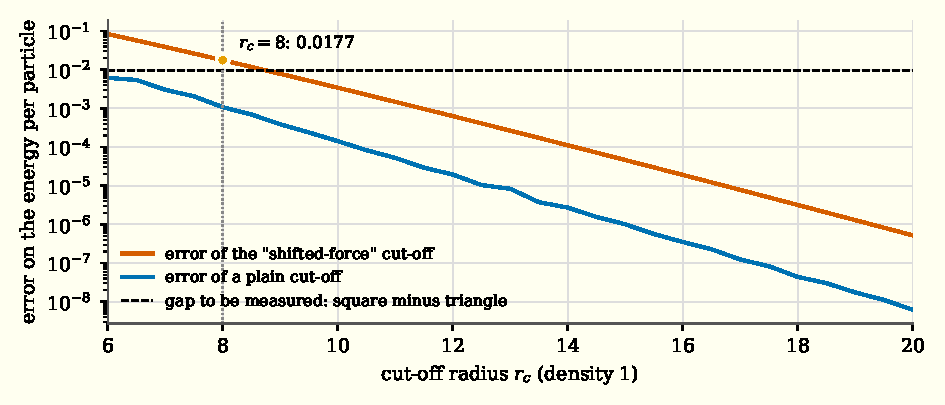
\includegraphics[width=\linewidth]{figures/c04_coupure}
\caption{Error on the energy per particle of the triangular lattice ($\kappa=1$) as a function of the cut-off radius,
recomputed by direct sums and compared with the square--triangle gap.}
\label{fig:c04}
\end{figure}

\section*{How we made sure it is not wrong}

\niveau{A} \emph{The judge looked.} Lean, the program that checks every step of a proof, accepted the two files with
only the three basic assumptions accepted everywhere; a proof left blank and an invented axiom, planted on purpose,
were detected; the two modules were replayed without error by a second checking program on 26 October 2026. An
independent AI agent recompiled exact copies of the files, planted its own traps, checked step by step the proof
written for humans, and gave a favourable opinion with five wording corrections, all applied; no statement and no
number changed. As everywhere in this book, no human specialist has reviewed these results, and the register of
claims flags this with 11 flags.

For the \niveau{X} calculations, an independent 40-digit check (another method, other code) recovers the exact
energies to within $1.7\times10^{-16}$. The test designed to fail fails: the old shifted-force values do not pass the
agreement check. And the square lattice remains an unstable saddle under the exact law.

\section*{What this does not say}

\begin{limite}
\begin{itemize}
\item Everything depends on the upstream theorem, produced by an AI and not yet reviewed by peers.
\item The law studied is the three-dimensional screened repulsion restricted to the plane; the purely
two-dimensional screening law is not treated.
\item Nothing about temperature, melting, or the path by which a real system reaches the lattice.
\item The new relaxations cover a subset of the published study (11 of 50 at $\kappa=1$, 13 of 100 at $\kappa=2$), and
the annealing was not redone.
\end{itemize}
\end{limite}

\section*{Going further}

This is a correction carried through to the end: the error in one paper is repaired in another, inside the same
audited loop. Paper: doi:10.5281/zenodo.23646105.
